%!TEX root = ../thesis.tex
% ******************************* Thesis Appendix A ****************************
\chapter{Supporting work for \autoref*{chap:denovo}}

\section{Length of missing loci in simulations}
\label{app:denovo-missing-lengths}

\autoref{fig:denovo-missing-len} shows the distribution of lengths for the missing loci in \autoref{sec:denovo-sims}. The most commonly missed locus was \vrb{GC00000093\_18}, which has a length of 146bp.

\begin{figure}
    \centering
    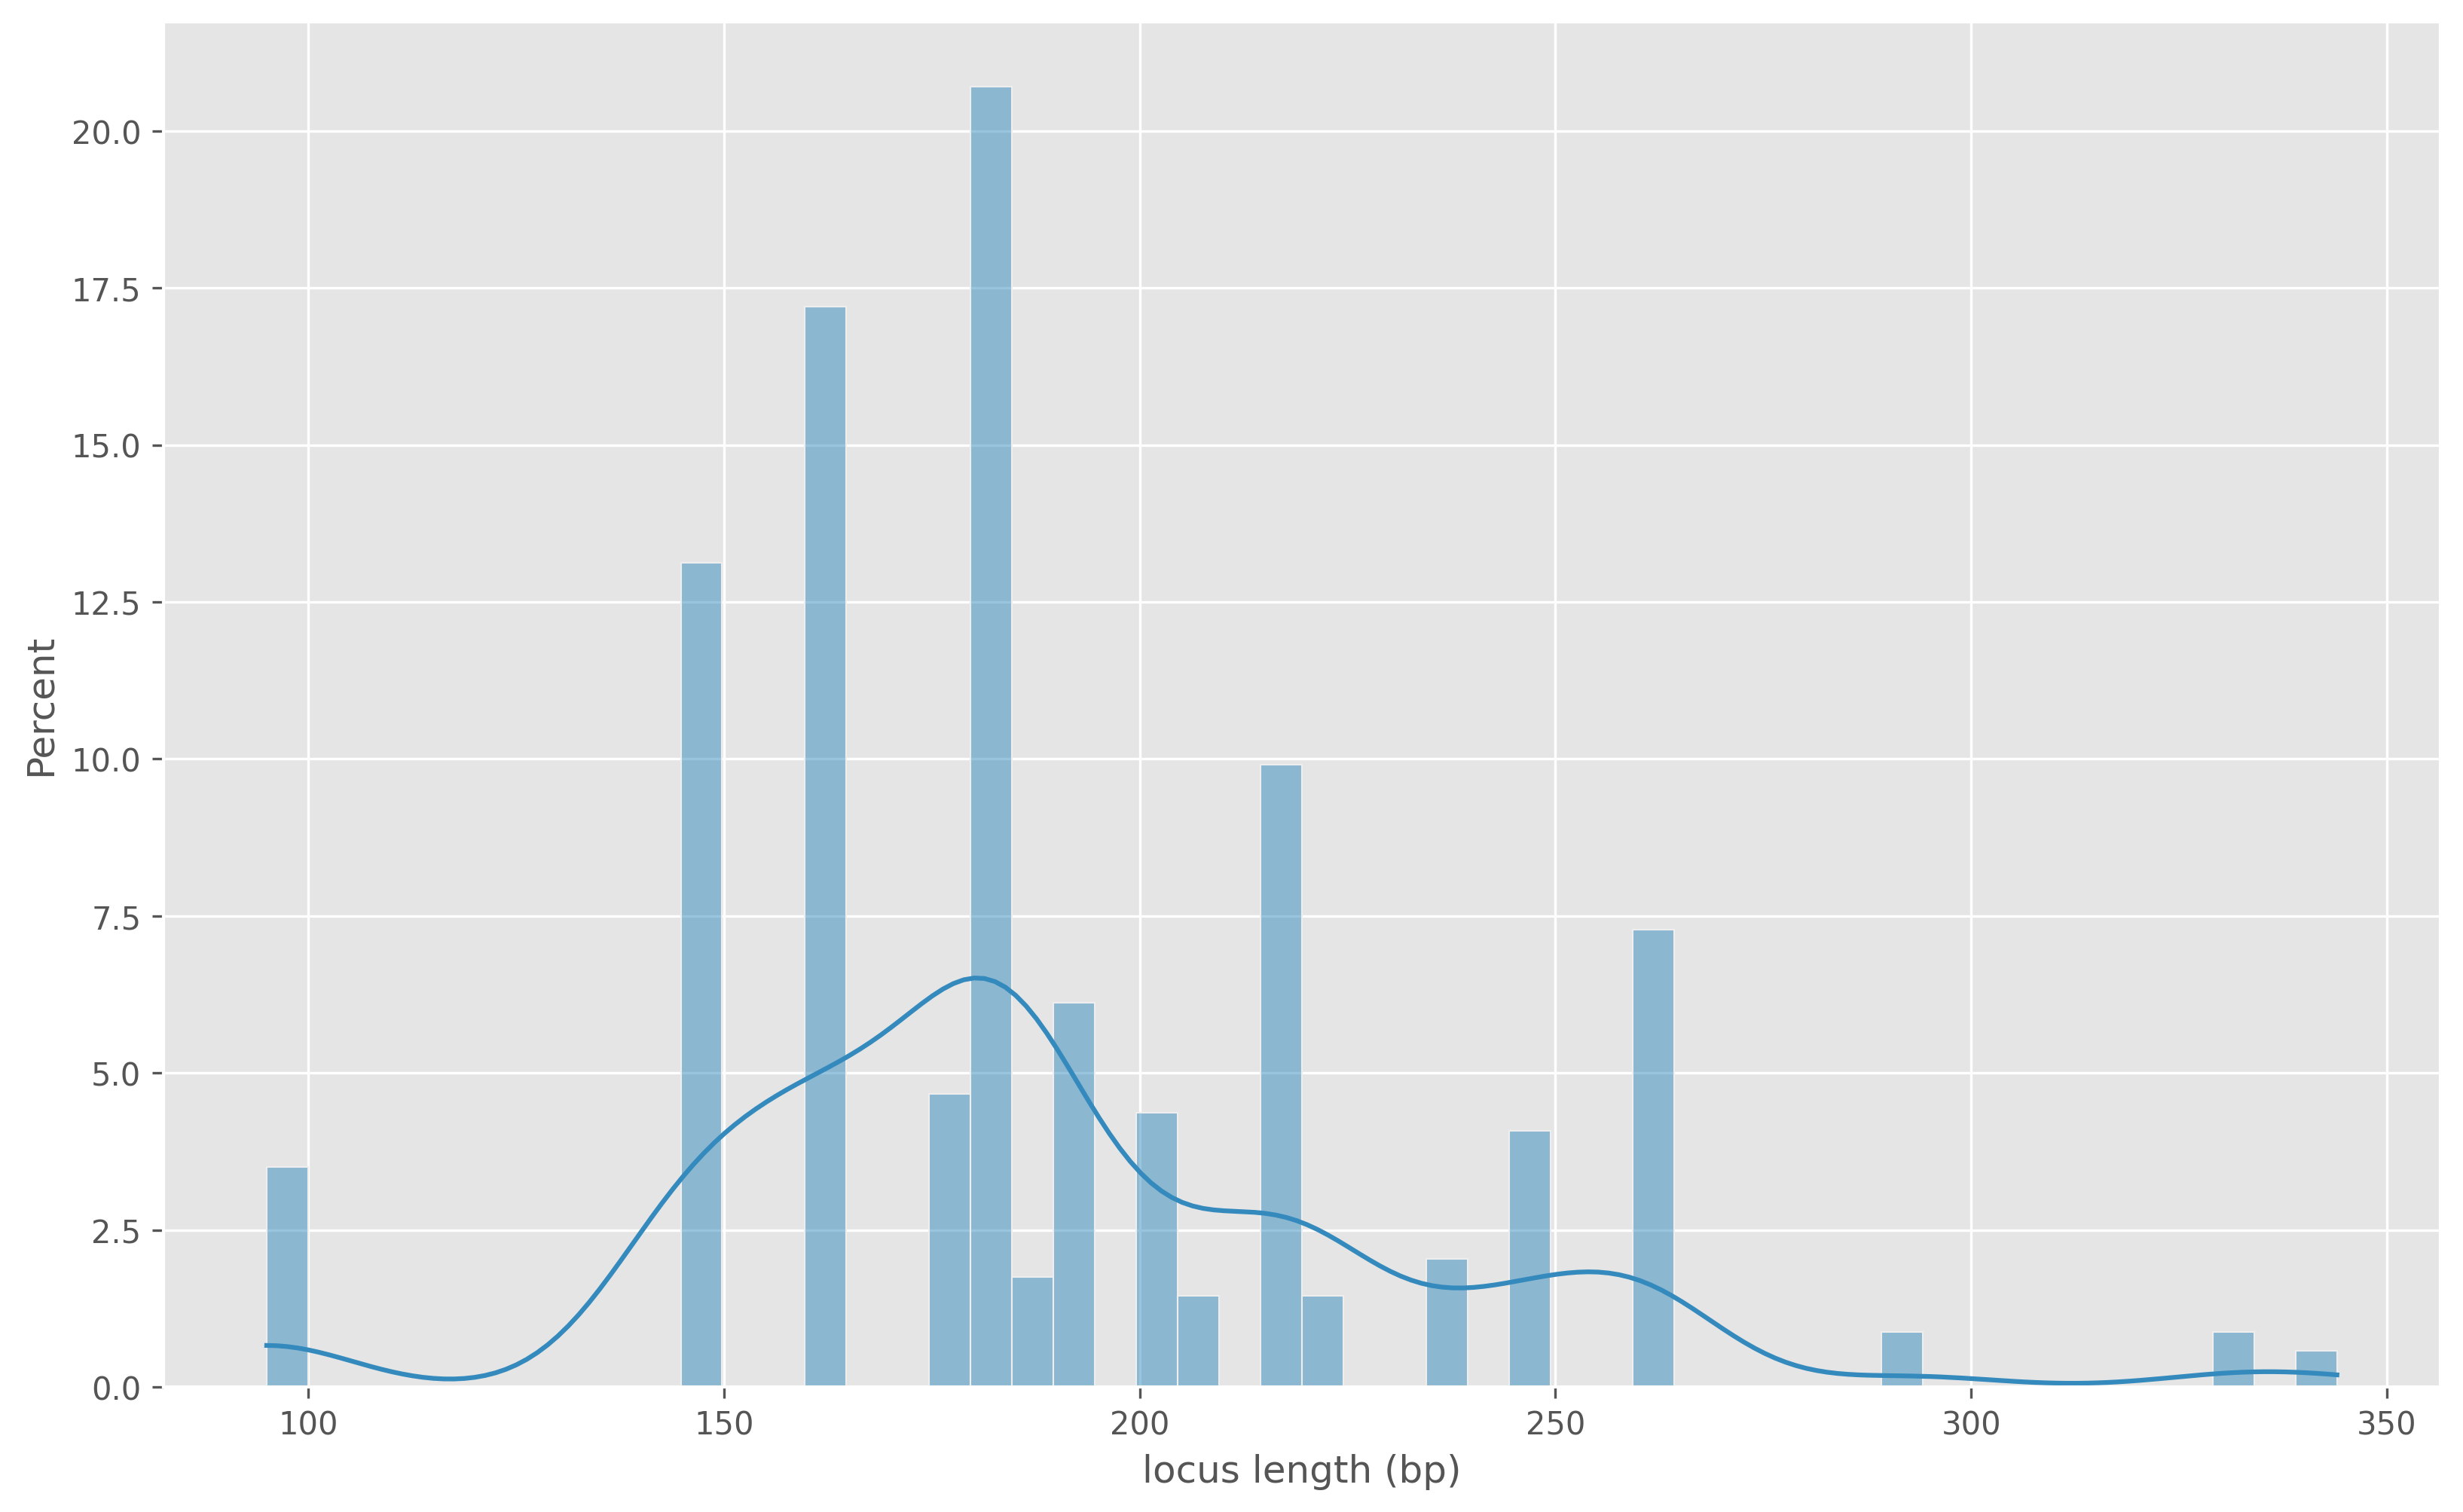
\includegraphics[width=0.9\textwidth]{Appendix0/Figs/denovo_missing_lengths.png}
    \caption{The lengths (x-axis; base pairs) of missing loci in the \denovo{} simulations in \autoref{sec:denovo-sims}}
    \label{fig:denovo-missing-len}
\end{figure}

% =====================================
\section{Constructing a pan-genome SNP truth set}
\label{app:pangenome-snp-truth}

\textit{The work in this section was performed by Leandro Ishi and is described here to aid the reader's understanding of the evaluation in \autoref{sec:denovo-empirical}. It is also described in detail in \cite{pandora}.}

The purpose of a truth set of pan-genome SNPs is to describe the variation that exists \emph{between} a collection of samples, rather than just between a single sample and a reference genome. Thus, for example, in the traditional model where a single reference genome is used to call variants for a collection of samples, if a gene that occurs in some of the samples does not occur in the reference genome used, there would be no recall penalty (see \autoref{fig:reference-bias}).

We first identify all pairwise differences between the 20 samples in this study (\autoref{sec:denovo-empirical-data}) with \vrb{dnadiff} \cite{mummer2018} and \vrb{minimap2} \cite{li2018}. We join these two sets of SNP differences and create a probe of each SNP with 50bp of flanking sequence from one of the genomes in the pairwise comparison. This probe is then mapped to the other genome, and if it maps to multiple locations or the allele does not perfectly match the sequence it aligns to, we remove it, ensuring our truth set is unambiguous.

These filtered pairwise variants ($PwV$) are then grouped into pan-genome variants ($PgV$). For instance, a variant between two genomes could be the same as a variant that exists between two different genomes, making it the same variant in the context of a pan-genome.

Each allele is uniquely defined as $A=(G_A,C_A,P_A)$, where $G_A$, $C_A$ and $P_A$ are the genome, chromosome, and position that the allele occurs in, respectively. Thus, a pairwise variant is formally described as an allele, $A$, between two genomes - $PwV=\{A_1,A_2\}$. Lastly, we define a pan-genome variant $PgV=\{PwV_1,PwV_2,...,PwV_n\}$. That is, if two pairwise variants $PwV_1$ and $PwV_2$ share an allele $A_i$, they are in the same pan-genome variant, $PgV$. Given the removal of multi-mapping probes, we also know that a $PwV$ can only occur in one $PgV$.

The truth set of pan-genome variants, $P$, is constructed using an undirected graph $G=(V,E)$, where $V$ is a set of nodes (pairwise variants ($PwV$)), and $E$ is a set of edges connecting two nodes if they share an allele. Therefore, a pan-genome variant, $PgV$, is a connected component (subgraph) $C \in G$, such that there exists a path between any two nodes ($PwV$) in $C$.

Finally, the pan-genome variants (connected components, $C$; $PgV$) are filtered such that a $PgV$ has no more than one allele ($A$) originating from the same genome, $G_A$, and can only be biallelic. Thus, in the end, each pan-genome variant describes the same variant in different genomes, letting go of a coordinate system; we find 618,305 such variants between the 20 samples.

\noindent
There are two measures of recall within such a pan-genome variant set: average allelic recall (AvgAR) and pan-variant recall (PVR). AvgAR is an average of the recall for all $PgV$s. That is, it describes what proportion of \emph{all} alleles in a $PgV$ are correctly discovered, averaged over all $PgV$s. In contrast, PVR is the proportion of $PgV$s where at least one allele was found. For example, we have two $PgV$s,  $V_1$, which contains two alleles present in 5 genomes each, and $V_2$, which has two alleles present in one genome each. If 8/10 alleles in $V_1$ and 0/2 alleles in $V_2$ are discovered, the AvgAR would be $\frac{(8/10)+(0/2)}{2}=0.4$ and PVR would be $\frac{1+0}{2}=0.5$.